% here live the intros to all the individual chapters
% also, you can toggle the inclusion of the individual 
% chapters (by commenting the \input{ch_c1.txt}) for a 
% faster build of the document during preparation

% use the brackets [] to use different formating in the text vs. the TOC 
\chapter[This is the very very, oh sooo very long title of Chapter 1 --- it even needs line breaks]{\centering This is the very very, oh sooo very long\\ title of Chapter1 --- it even needs line breaks}
\vfill

\chapterauthor{\textbf{First Author}}{1}{,}{1.3}{,}
\chapterauthor{Second Author}{2}{,}{0}{,}
\chapterauthor{Third Author}{3}{, \smallskip}{0}{,}
\chapterauthor{Fourth Author}{1}{\vspace*{-.5em}\\}{0}{}

\noindent\begin{tabular}{L{.015\textwidth}L{.985\textwidth}}
    1 & First Research Institute \\
    2 & Second Research Institute \\
    3 & Third Research Institute
\end{tabular}

\noindent\colorbox{clrt1!15}{\parbox{\textwidth}{
This study was originally published in \textit{Name of the Journal}.
Figures were re-drawn for this thesis but no additional changes were made.
The re-print within this thesis is in agreement with \textit{Name of the Publisher} under license number \textit{XX}.

\nociteat{ref1}
\bibliographystyleat{apalikeK}
\bibliographyat{library/chapters.bib}
}}

\noindent\section*{Abstract}
This includes a demo of a Supplementary Figure, the \textit{narrow mode} which works for Figures and Supplementary Figure and use a chapter-specific citation.

\noindent{\bf Keywords:} Key1, Key2, Key3.

\begin{multicols}{2}
\section{Introduction}
\noindent
Here again, we showcase some old stuff that needs a (chapter-specific) citation \citepam{Darwin1859}.
Also, note the slight variation in referencing Supplementary Figures (\figrefS{fig:c1s1}) using \textsw{$\backslash figrefS\{\}$} (vs. \textsw{$\backslash figref\{\}$}).
Then again, it is time for dummy text: 

\section{A section}
% demo of a supplementary figure (in "narrow mode" )
\begin{supplFigure*}[!t]
\floatbox[{\capbeside\thisfloatsetup{capbesideposition={left,center},capbesidewidth=.5\fwidth}}]{supplFigure}[\FBwidth]
{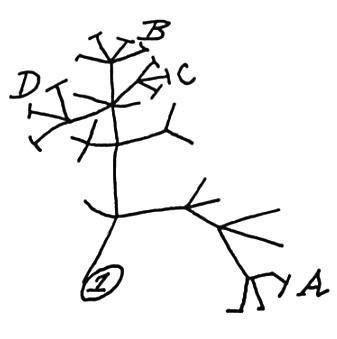
\includegraphics[width = .5\fwidth]{figures/c1/tree.jpg}}
{\caption[Darwins tree]{\label{fig:c1s1}\textbf{Darwins tree.}
Oh, the fame...}}
\end{supplFigure*}


\lipsum[2-6] 

\bibliographystyleam{apalike}
\bibliographyam{library/c1.bib}
\end{multicols}

\chapter[Short title of Chapter 2]{\centering Short title of Chapter 2\\}

\chapterauthor{\textbf{First Author}}{1}{,}{1.3}{,}
\chapterauthor{Second Author}{2}{,}{0}{,}
\chapterauthor{Third Author}{3}{, \smallskip}{0}{,}

\noindent\begin{tabular}{L{.015\textwidth}L{.985\textwidth}}
    1 & First Research Institute \\
    2 & Second Research Institute \\
    3 & Third Research Institute
\end{tabular}

\noindent\colorbox{clrt1!15}{\parbox{\textwidth}{
This study was originally published in \textit{Name of the Journal}.
Figures were re-drawn for this thesis but no additional changes were made.
The re-print within this thesis is in agreement with \textit{Name of the Publisher} as the original publication is under Creative Commons CC BY license.

\nocitebt{ref2}
\bibliographystylebt{apalikeK}
\bibliographybt{library/chapters.bib}
}}

\section*{Abstract}
\noindent
Here, we talk about different citation styles and look at tabels.

\noindent{\bf Keywords:} Key1, key2, key3.

\begin{multicols}{2}

\begin{table*}[!htb]
\centering
\caption[Summary of Anderson's Iris Data]{\label{tab:c2t1}
A small summary of Edgar Anderson's Iris Data as implemented in R.}
\begin{small}
\arrayrulecolor{black!25}
\begin{tabular}{ r | c c | c c }
\arrayrulecolor{black}
\hline
\arrayrulecolor{black!25}
\multirow{2}{*}{\textbf{Species}} &\multicolumn{2}{c|}{\textbf{Sepal}}&\multicolumn{2}{c}{\textbf{Petal}}\\
& \textbf{Avg. Length} & \textbf{Avg. Width} & \textbf{Avg. Length} & \textbf{Avg. Width}\\
\arrayrulecolor{black}\hline
\textit{I. setosa}&5.01&3.428&1.46&0.246\\
\textit{I. versicolor}&5.94&2.77&4.26&1.33\\
\textit{I. irginica}&6.59&2.974&5.55&2.03\\\hline\hline
\end{tabular}

\end{small}
\end{table*}

\section{Introduction}

So, as far as citations go, I use a modular command system: This is based on the basic \LaTeX - citation commands (\textsw{$\backslash cite$}, \textsw{$\backslash citep$} and \textsw{$\backslash citealt$}) and two single-letter suffixes (i/a/b/c/d/z and t/m). The first letter indicates the current section (Intro: I, Chapter 1:a, 2:b, Synthesis:z), while the last letter indicates whether this is the self-citation from the Chapter title page (t) or a citation within the manuscript (m).
Form these pieces, the actual commands can be puzzled together, with the actual commands looking something like \textsw{$\backslash citepcm\{\}$}.

So, you might remember that in the first Chapter \citepbm{ref1}, we cited \citebm{Darwin1859} a lot.
Now in this chapter we are going to look at the data from \citealtbm{Anderson35}.
We are going to show a summary of this data in a main table (\tabref{tab:c2t1}), while a glimpse of the actual data structure is given in a Supplemental Table (\tabrefS{tab:c2st1}).
The referencing of the tables happens using the commands \textsw{$\backslash tabref\{\}$} and \textsw{$\backslash tabrefS\{\}$}.

\section{First Section}
\lipsum[7-9]

\begin{supplTable*}[!t]
\centering
\captionsetup{width=.6\linewidth}
\caption[Subset of Anderson's Iris Data]{\label{tab:c2st1}
A subset of Edgar Anderson's Iris Data as implemented in R.}
\begin{small}
\begin{tabular}{ r c c c c }
Species&Sepal Length&Sepal Width&Petal Length&Petal Width\\\hline
\textit{I. setosa}&5.4&3.4&1.7&0.2\\
\textit{I. setosa}&5.4&3.7&1.5&0.2\\
\textit{I. setosa}&5.7&3.8&1.7&0.3\\
\textit{I. setosa}&5.1&3.5&1.4&0.2\\
\textit{I. setosa}&4.8&3&1.4&0.3\\
\textit{I. setosa}&5.1&3.3&1.7&0.5\\\arrayrulecolor{black!25}\hline
\textit{I. versicolor}&5.8&2.6&4.0&1.2\\
\textit{I. versicolor}&5.8&2.7&3.9&1.2\\
\textit{I. versicolor}&5.5&2.3&4.0&1.3\\
\textit{I. versicolor}&6.0&2.7&5.1&1.6\\
\textit{I. versicolor}&5.6&3.0&4.5&1.5\\
\textit{I. versicolor}&6.3&3.3&4.7&1.6\\\hline
\textit{I. virginica}&6.9&3.2&5.7&2.3\\
\textit{I. virginica}&7.2&3.2&6.0&1.8\\
\textit{I. virginica}&6.5&3.0&5.5&1.8\\
\textit{I. virginica}&5.8&2.7&5.1&1.9\\
\textit{I. virginica}&6.3&3.4&5.6&2.4\\
\textit{I. virginica}&7.7&2.6&6.9&2.3\\\arrayrulecolor{black}\hline
\end{tabular}

\end{small}
\end{supplTable*}

\section{Second Section}
\lipsum[10-12]

\section*{Acknowledgments}

We thank all the nice people.

\bibliographystylebm{apalike}
\bibliographybm{library/c2.bib}
\end{multicols}

